
%  CONFIGURE NEW SINGLE-PAGE FORMAT 

\onecolumn % go back to one column
\fancyhead{} % make sure we get no headers
\renewcommand{\floatpagefraction}{0.1}
\lfoot[\bSupInf]{\dAuthor}
\rfoot[\dAuthor]{\cSupInf}
\newpage

\captionsetup*{format=largeformat} % make figure legend slightly larger than in the paper
\setcounter{figure}{0} % reset figure counter for Sup. Figures
\setcounter{equation}{0} % reset equation counter for Sup. Equations
\setcounter{table}{0} % reset equation counter for Sup. Equations
\setcounter{page}{1} % reset page count
\makeatletter
\renewcommand{\thefigure}{S\@arabic\c@figure} % make Figure legend start with Fig. S.
\makeatother
\makeatletter
\renewcommand{\thetable}{S\@arabic\c@table} % make Figure legend start with Fig. S.
\makeatother
\makeatletter
\renewcommand{\theequation}{S\@arabic\c@equation} % make Figure legend start with Fig. S.
\makeatother


\begin{figure*}[!t]
\centering
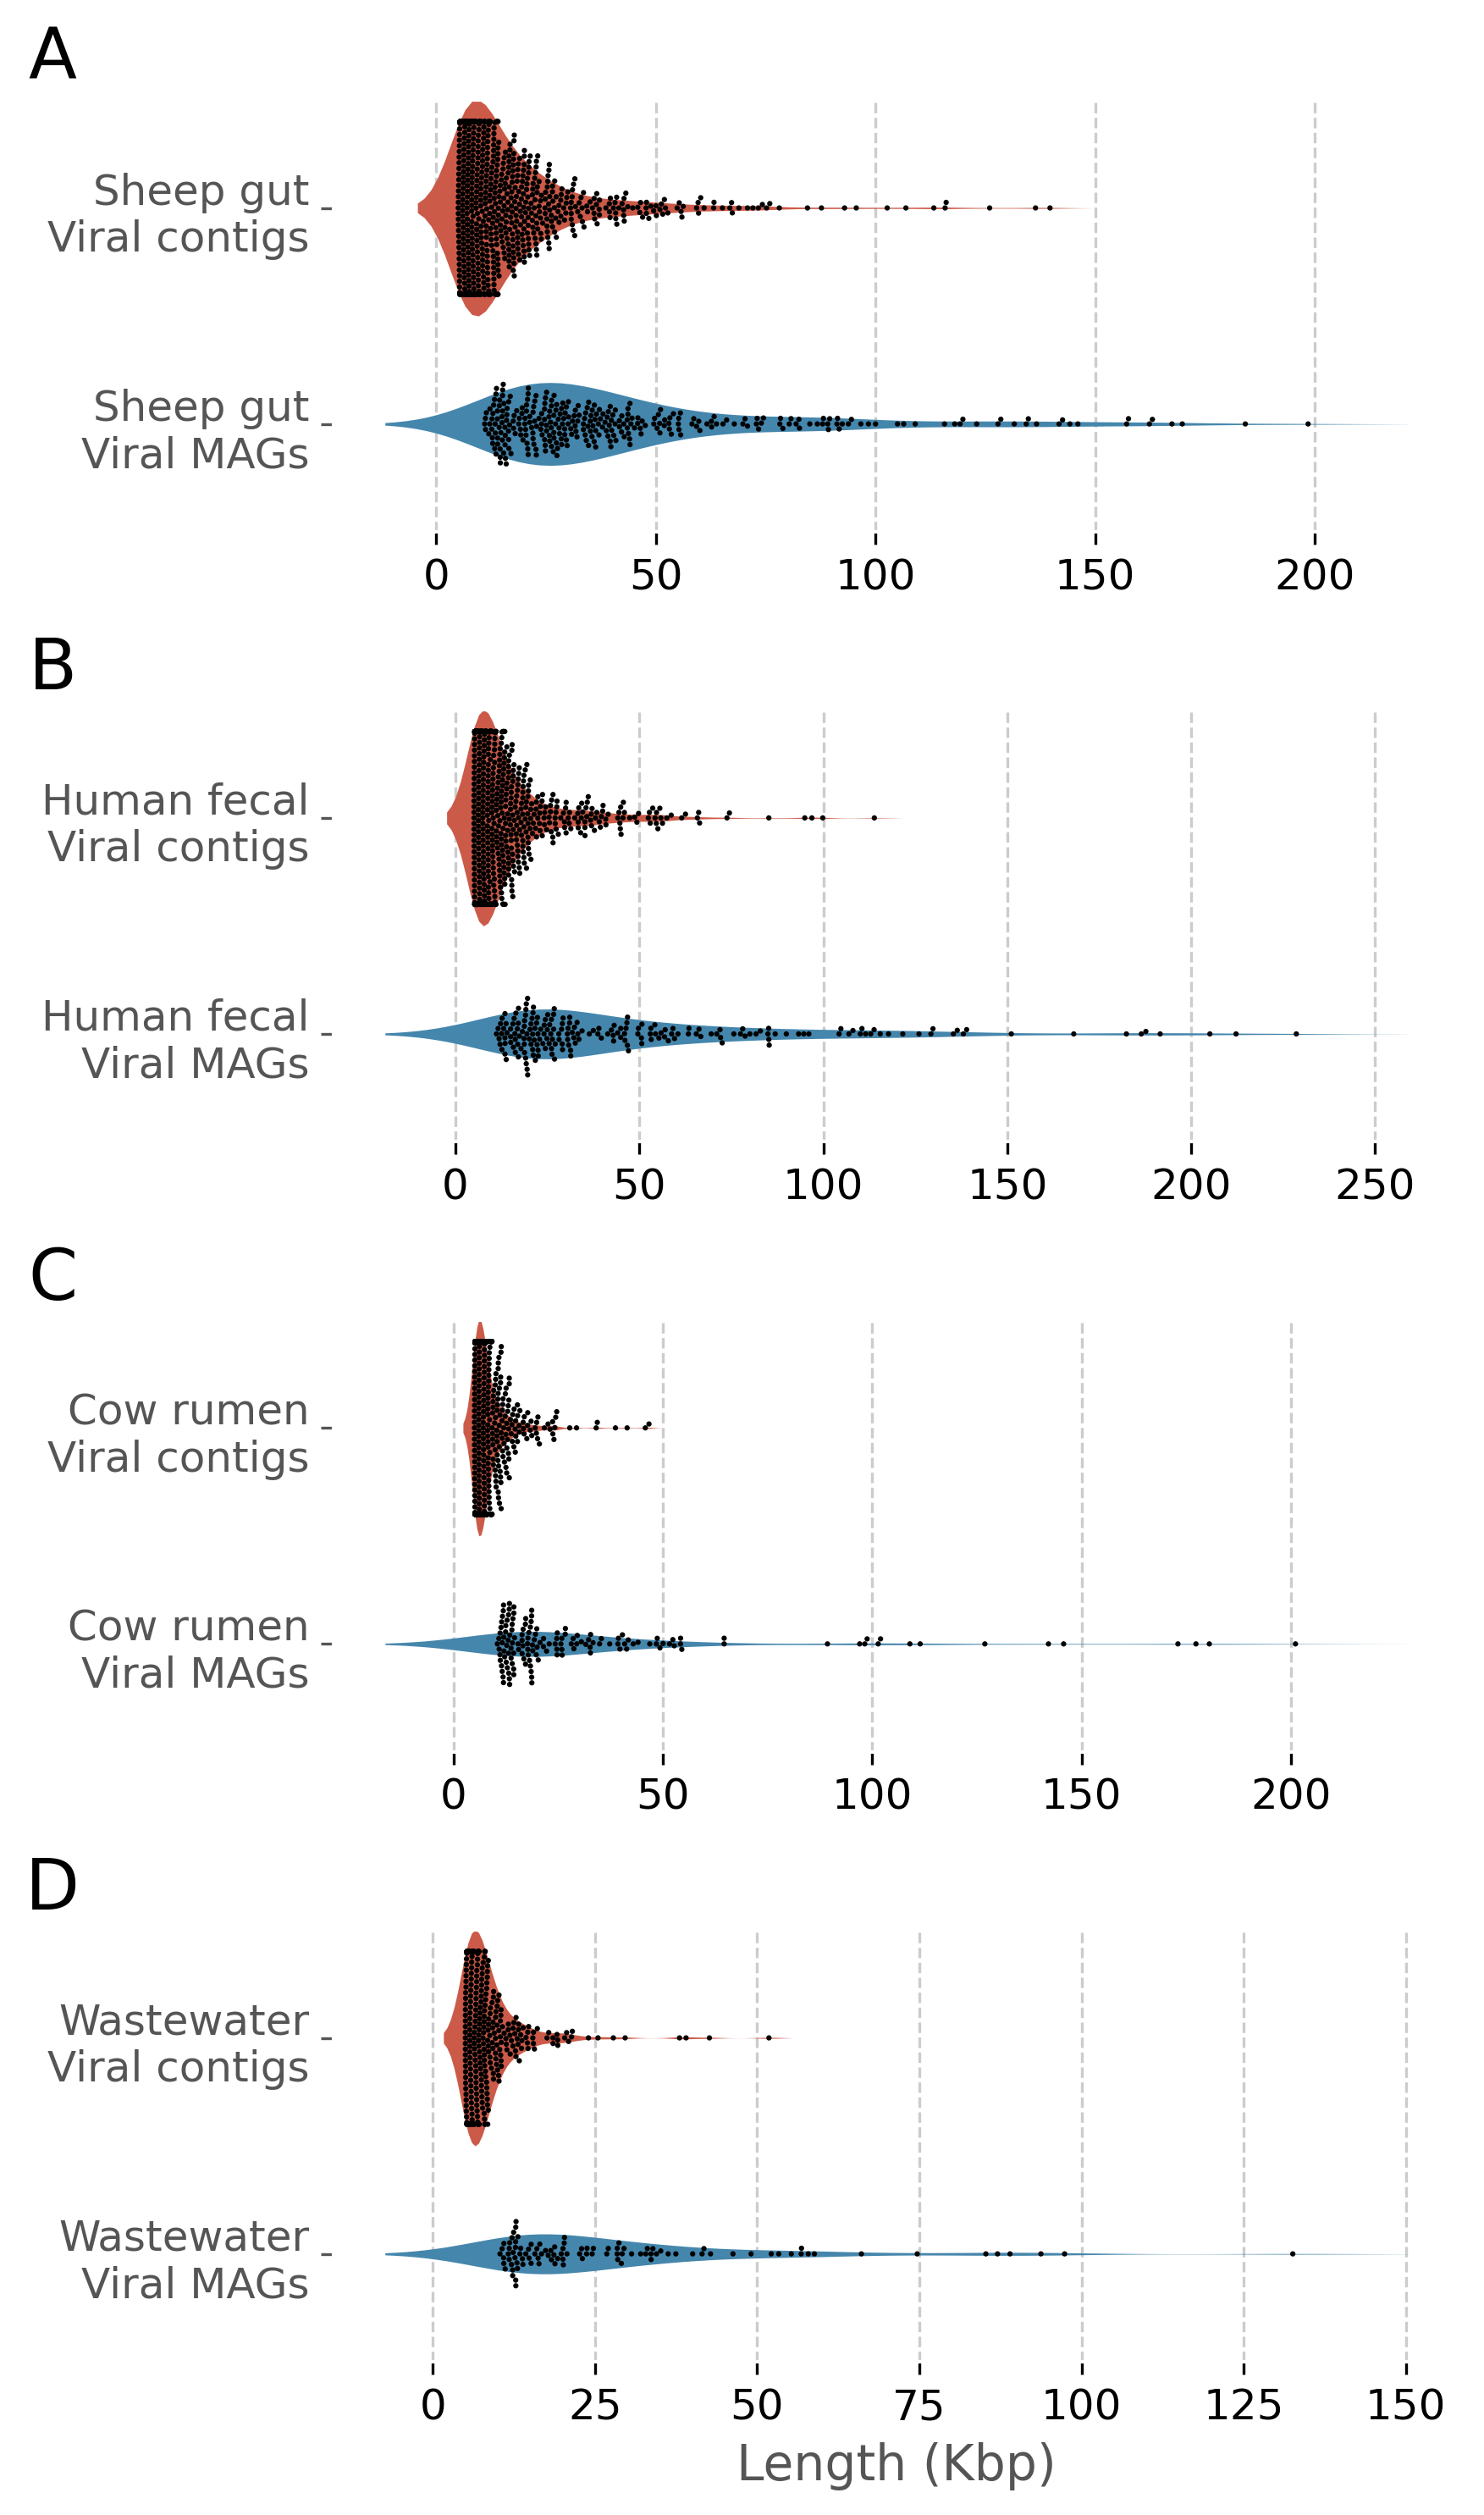
\includegraphics[scale=0.7]{Figures/figure_all_length_increases.png}
\caption{\textbf{Viral MAG lengths.} The length distribution of viral sequences before (red) and after (blue) binning with ProxiPhage in metagenomic samples extracted from A) sheep gut, B) human stool, C) cow rumen, and D) wastewater.}
\label{fig:figure_all_length_increases}
\end{figure*}
\newpage

\begin{figure*}[!t]
\centering
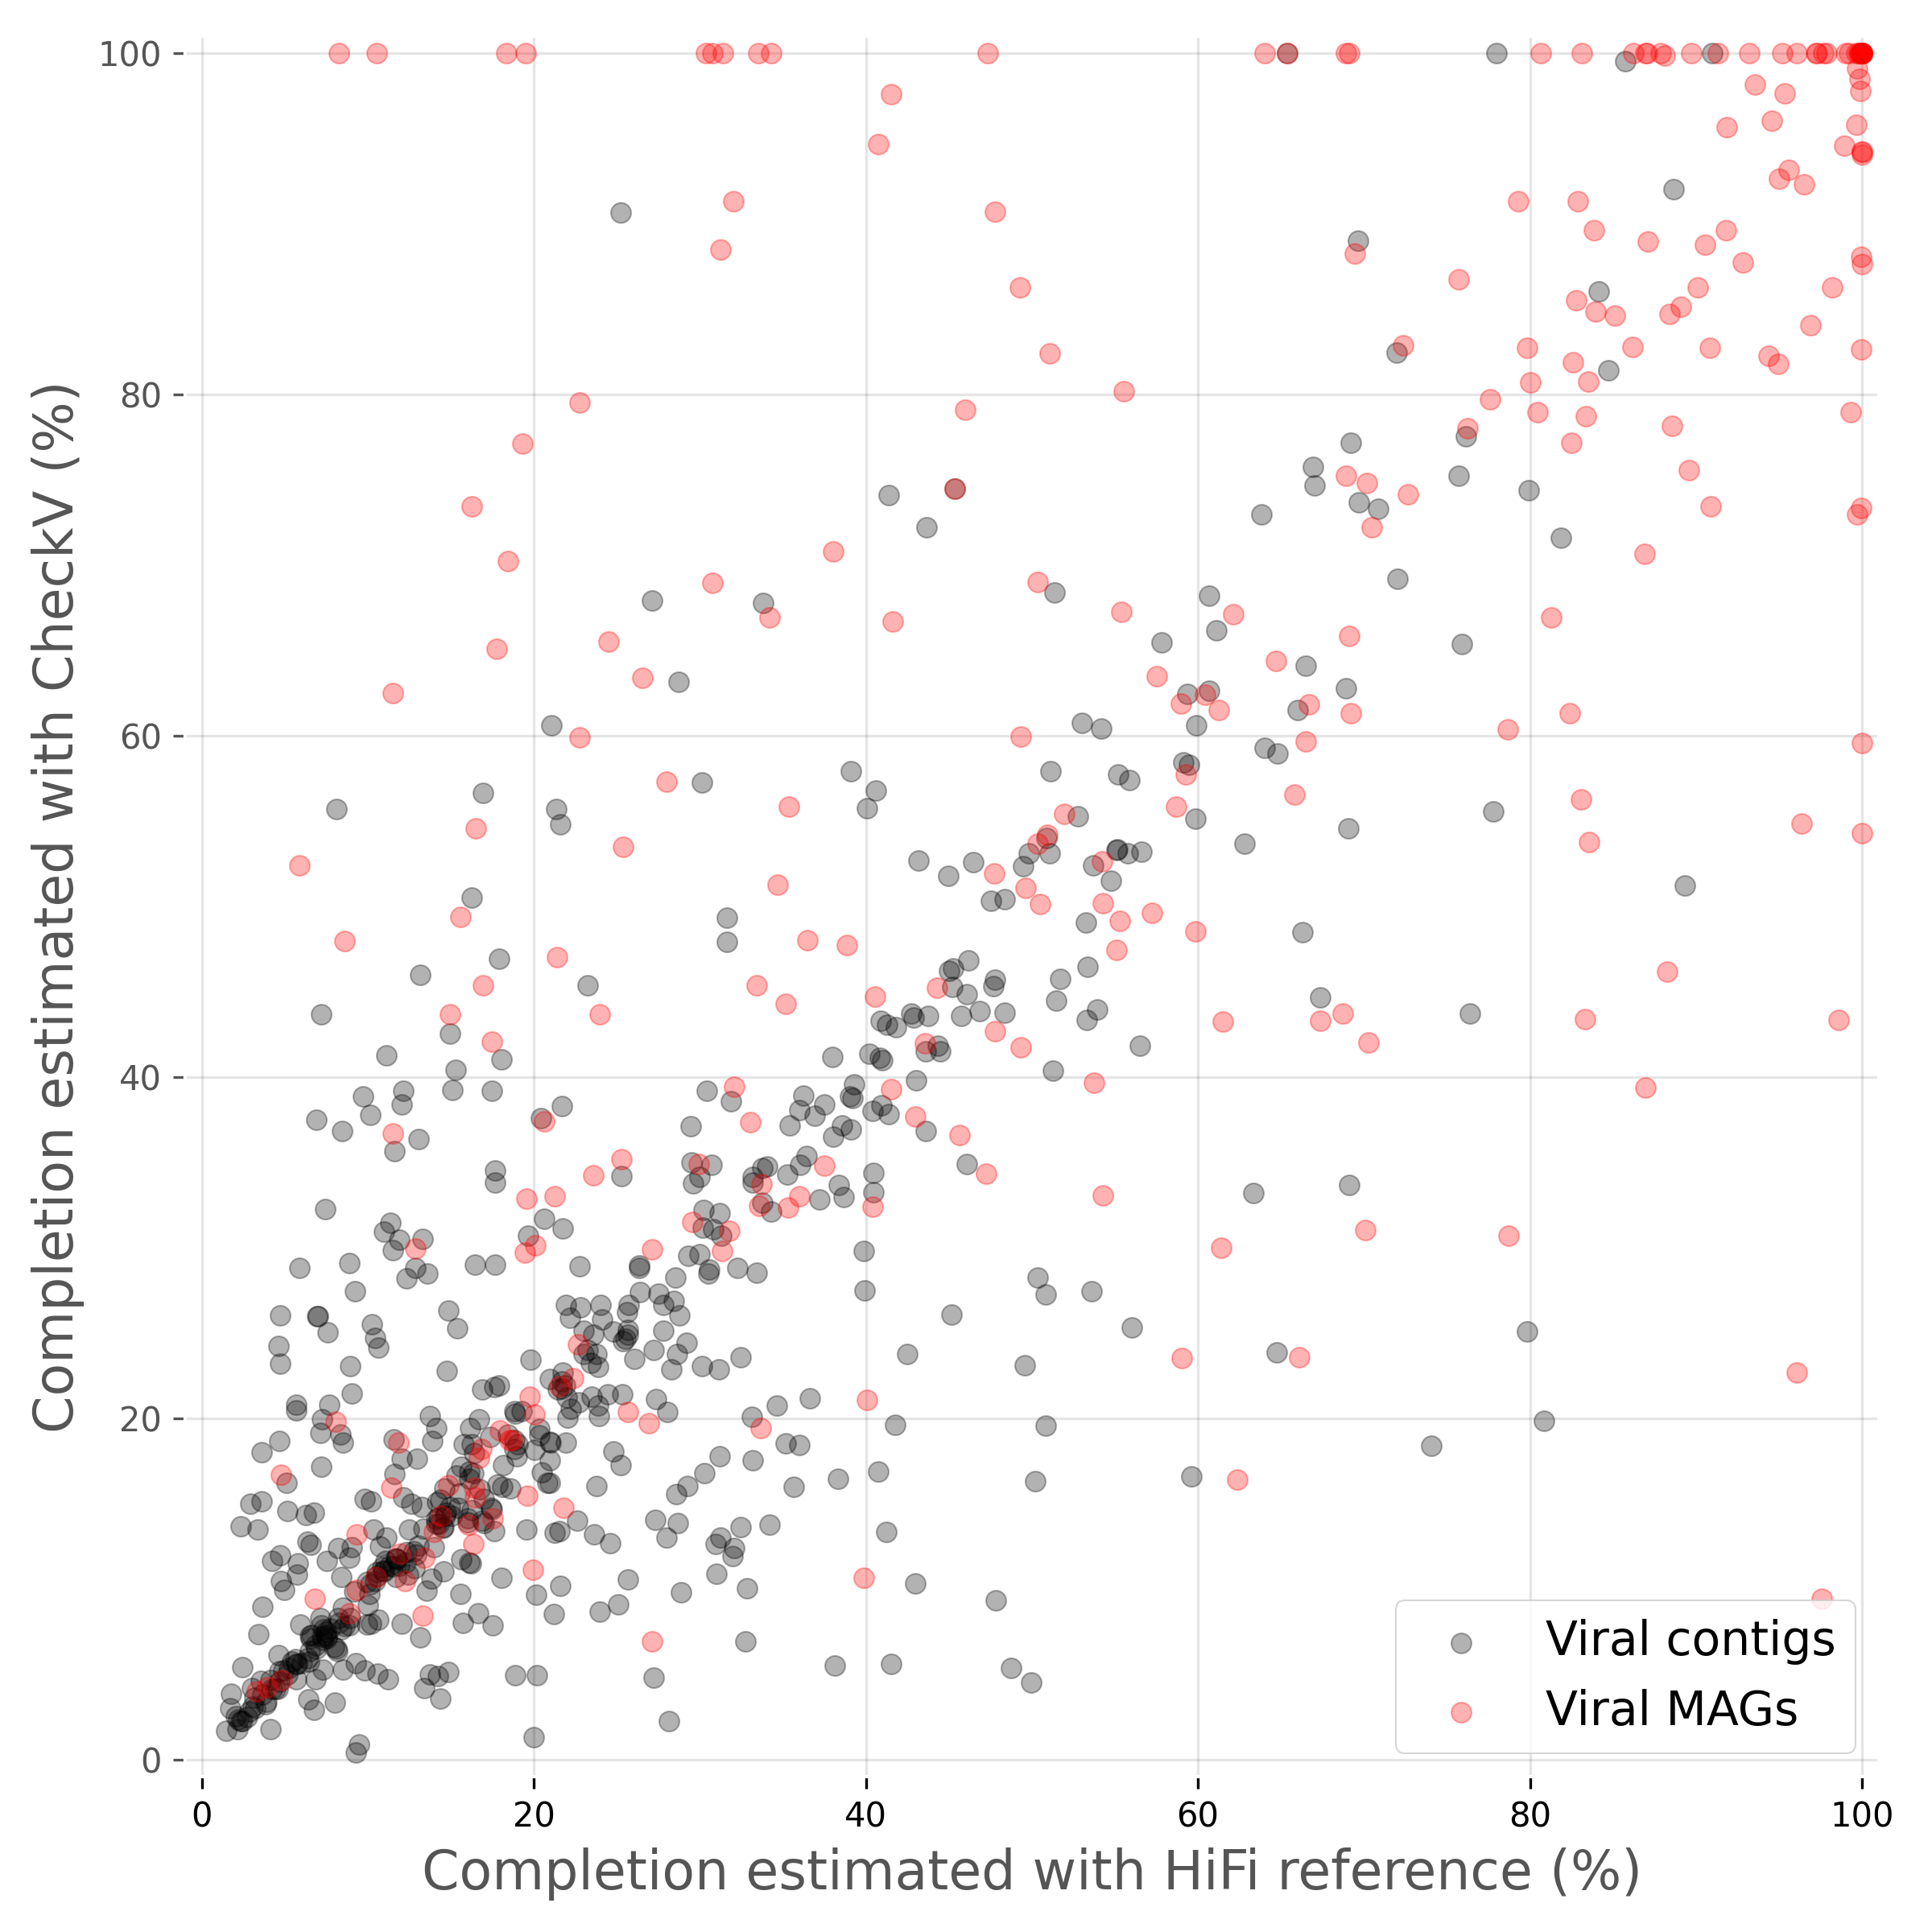
\includegraphics[scale=0.5]{Figures/figure_completion_checkv_vs_hifi.png}
\caption{\textbf{Completion estimation comparison.} Scatter plot of completion percentages of viral contigs and vMAGs from a sheep gut metagenome, estimated with CheckV (y-axis) and with reference excised phages from a long-read HiFi assembly (x-axis).}
\label{fig:figure_completion_checkv_vs_hifi}
\end{figure*}
\newpage

\begin{figure*}[!t]
\centering
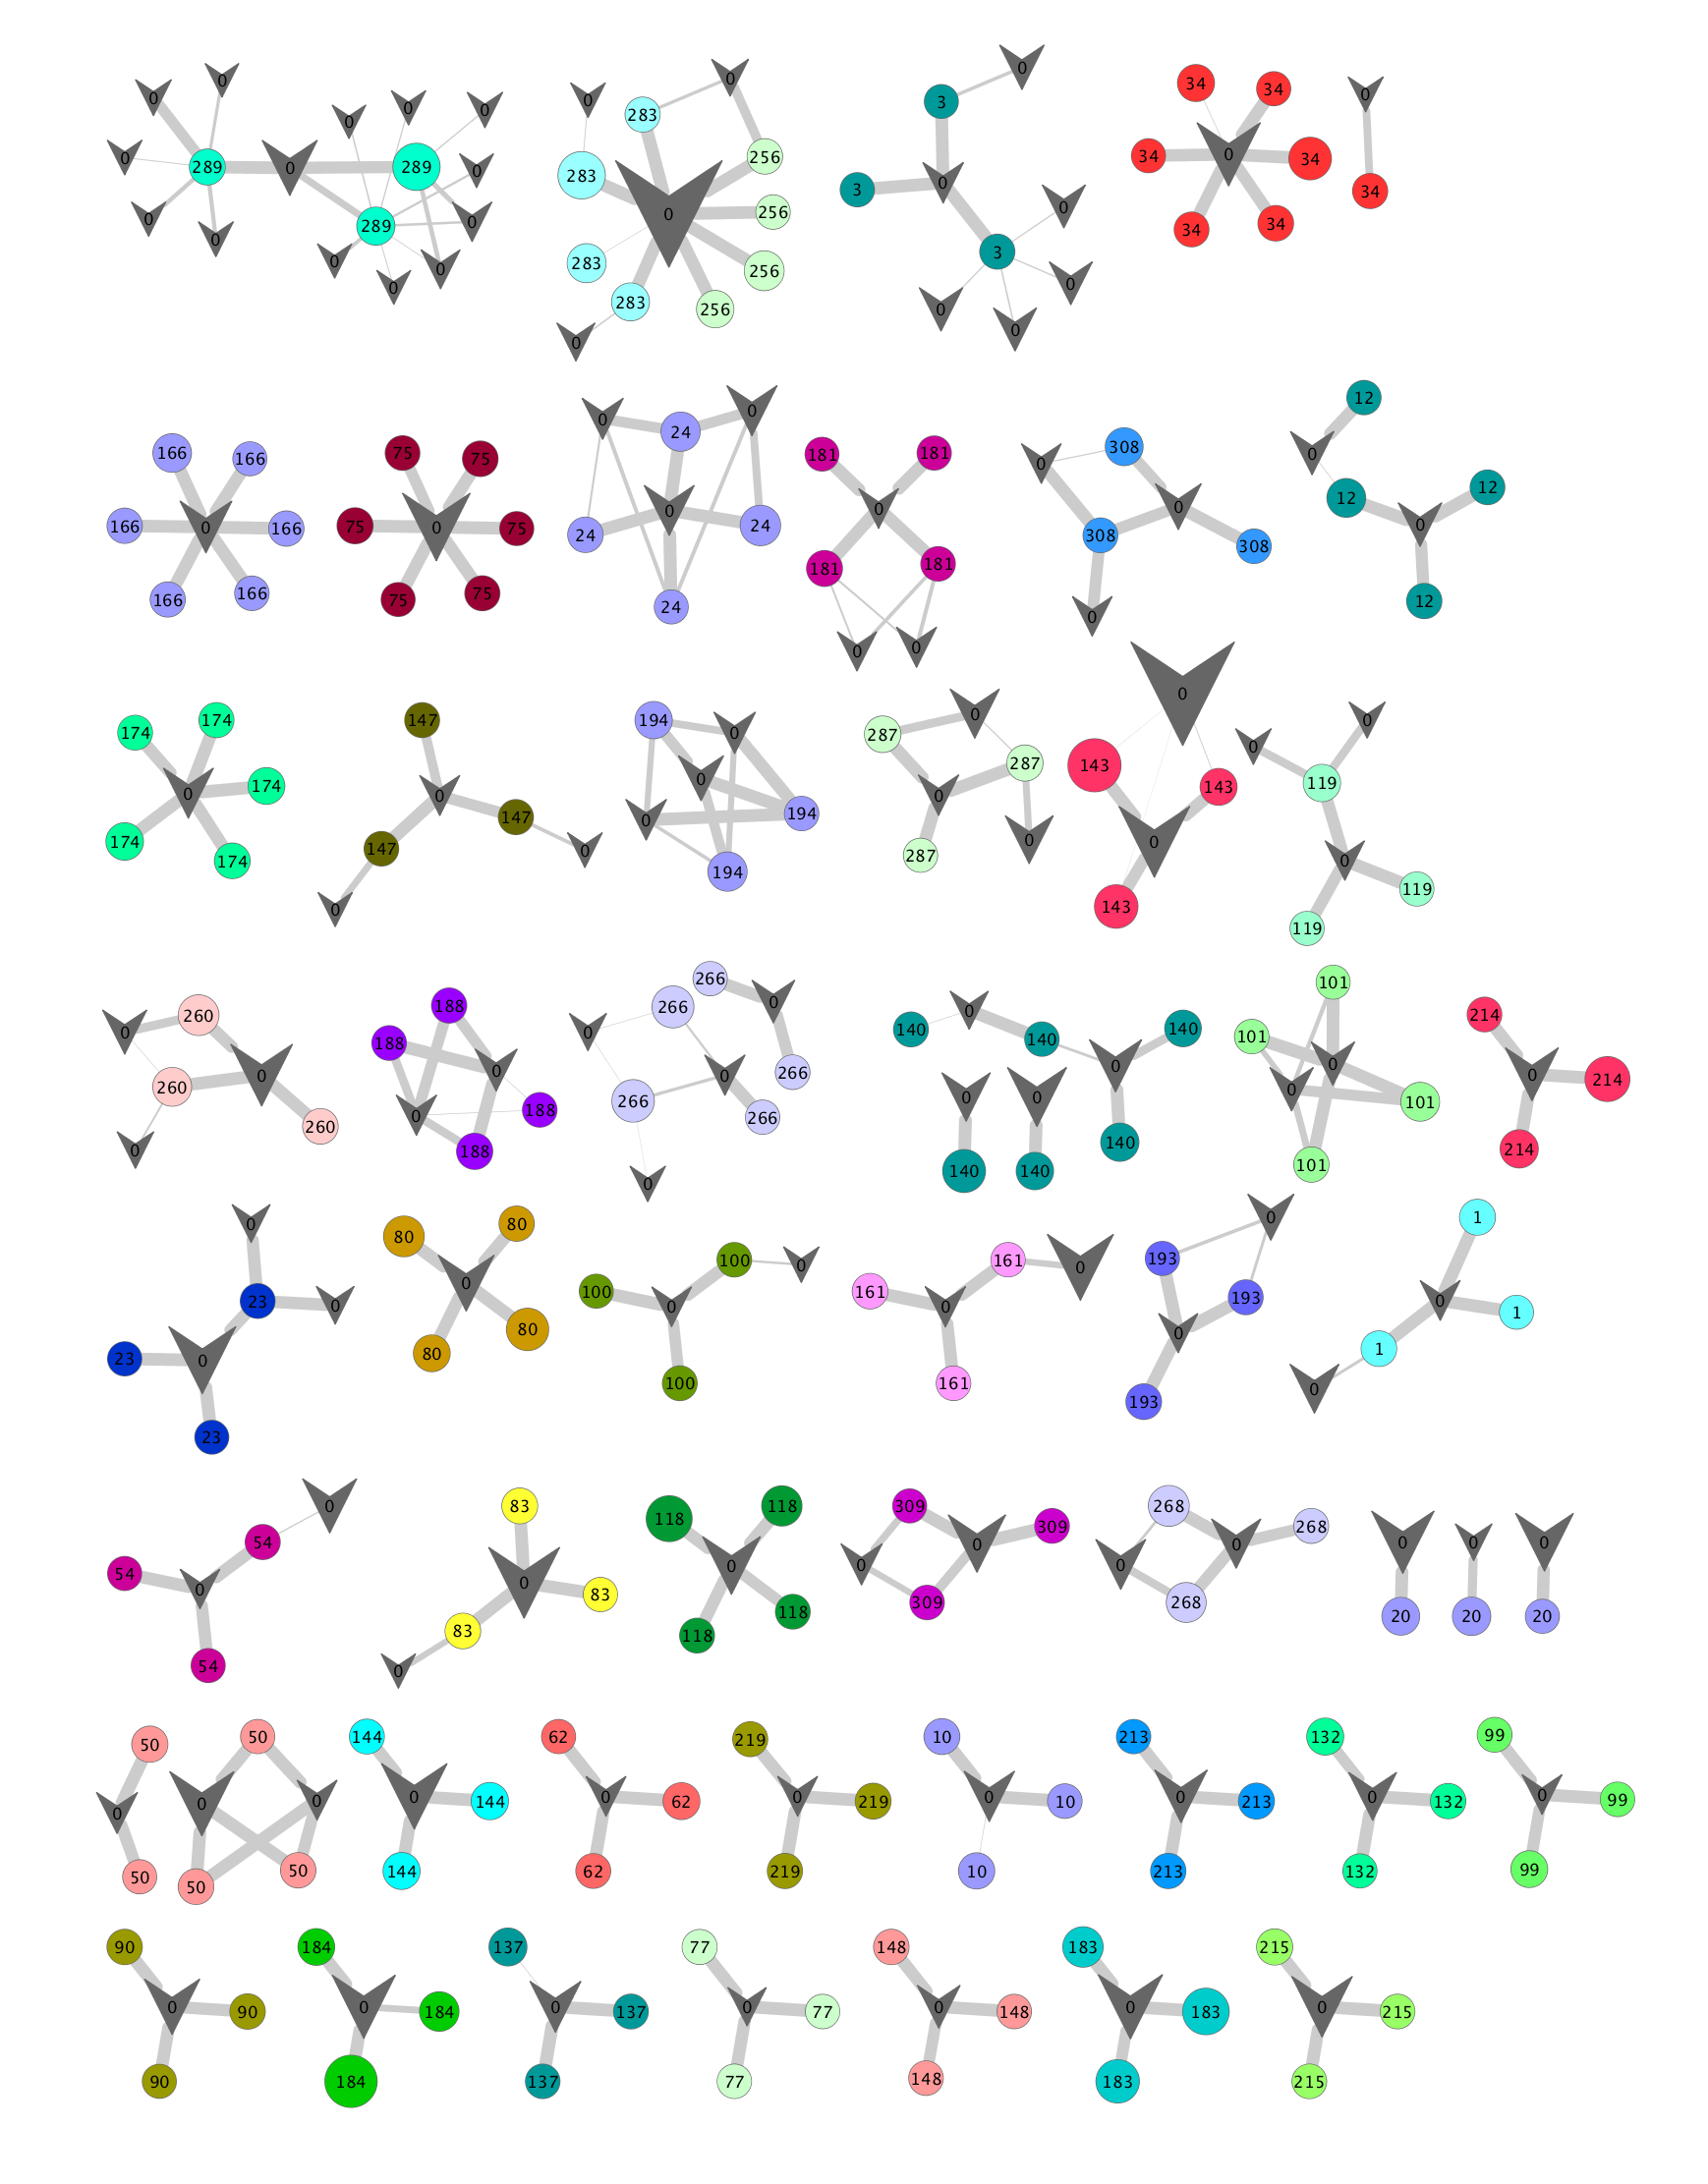
\includegraphics[scale=0.23]{Figures/figure_support_network.png}
\caption{\textbf{Viral MAG validation network.} Network showing long-read validation of vMAG contig clusters from a sheep gut metagenome. Viral contigs (circles, labeled with vMAG identifiers) are randomly colored according to the vMAG they belong to and linked to reference long-read viral genomes that they aligned to (grey check marks). The node size represents the viral sequence length, and the edge weight represents the percent of the short-read viral contig that aligned to the long-read reference. A random subset of 50 vMAGs was chosen for this visualization from a pool of vMAGs with at least 3 contigs and with at least one reference found for each contig.}
\label{fig:figure_support_network}
\end{figure*}
\newpage

\begin{figure*}[t]
\centering
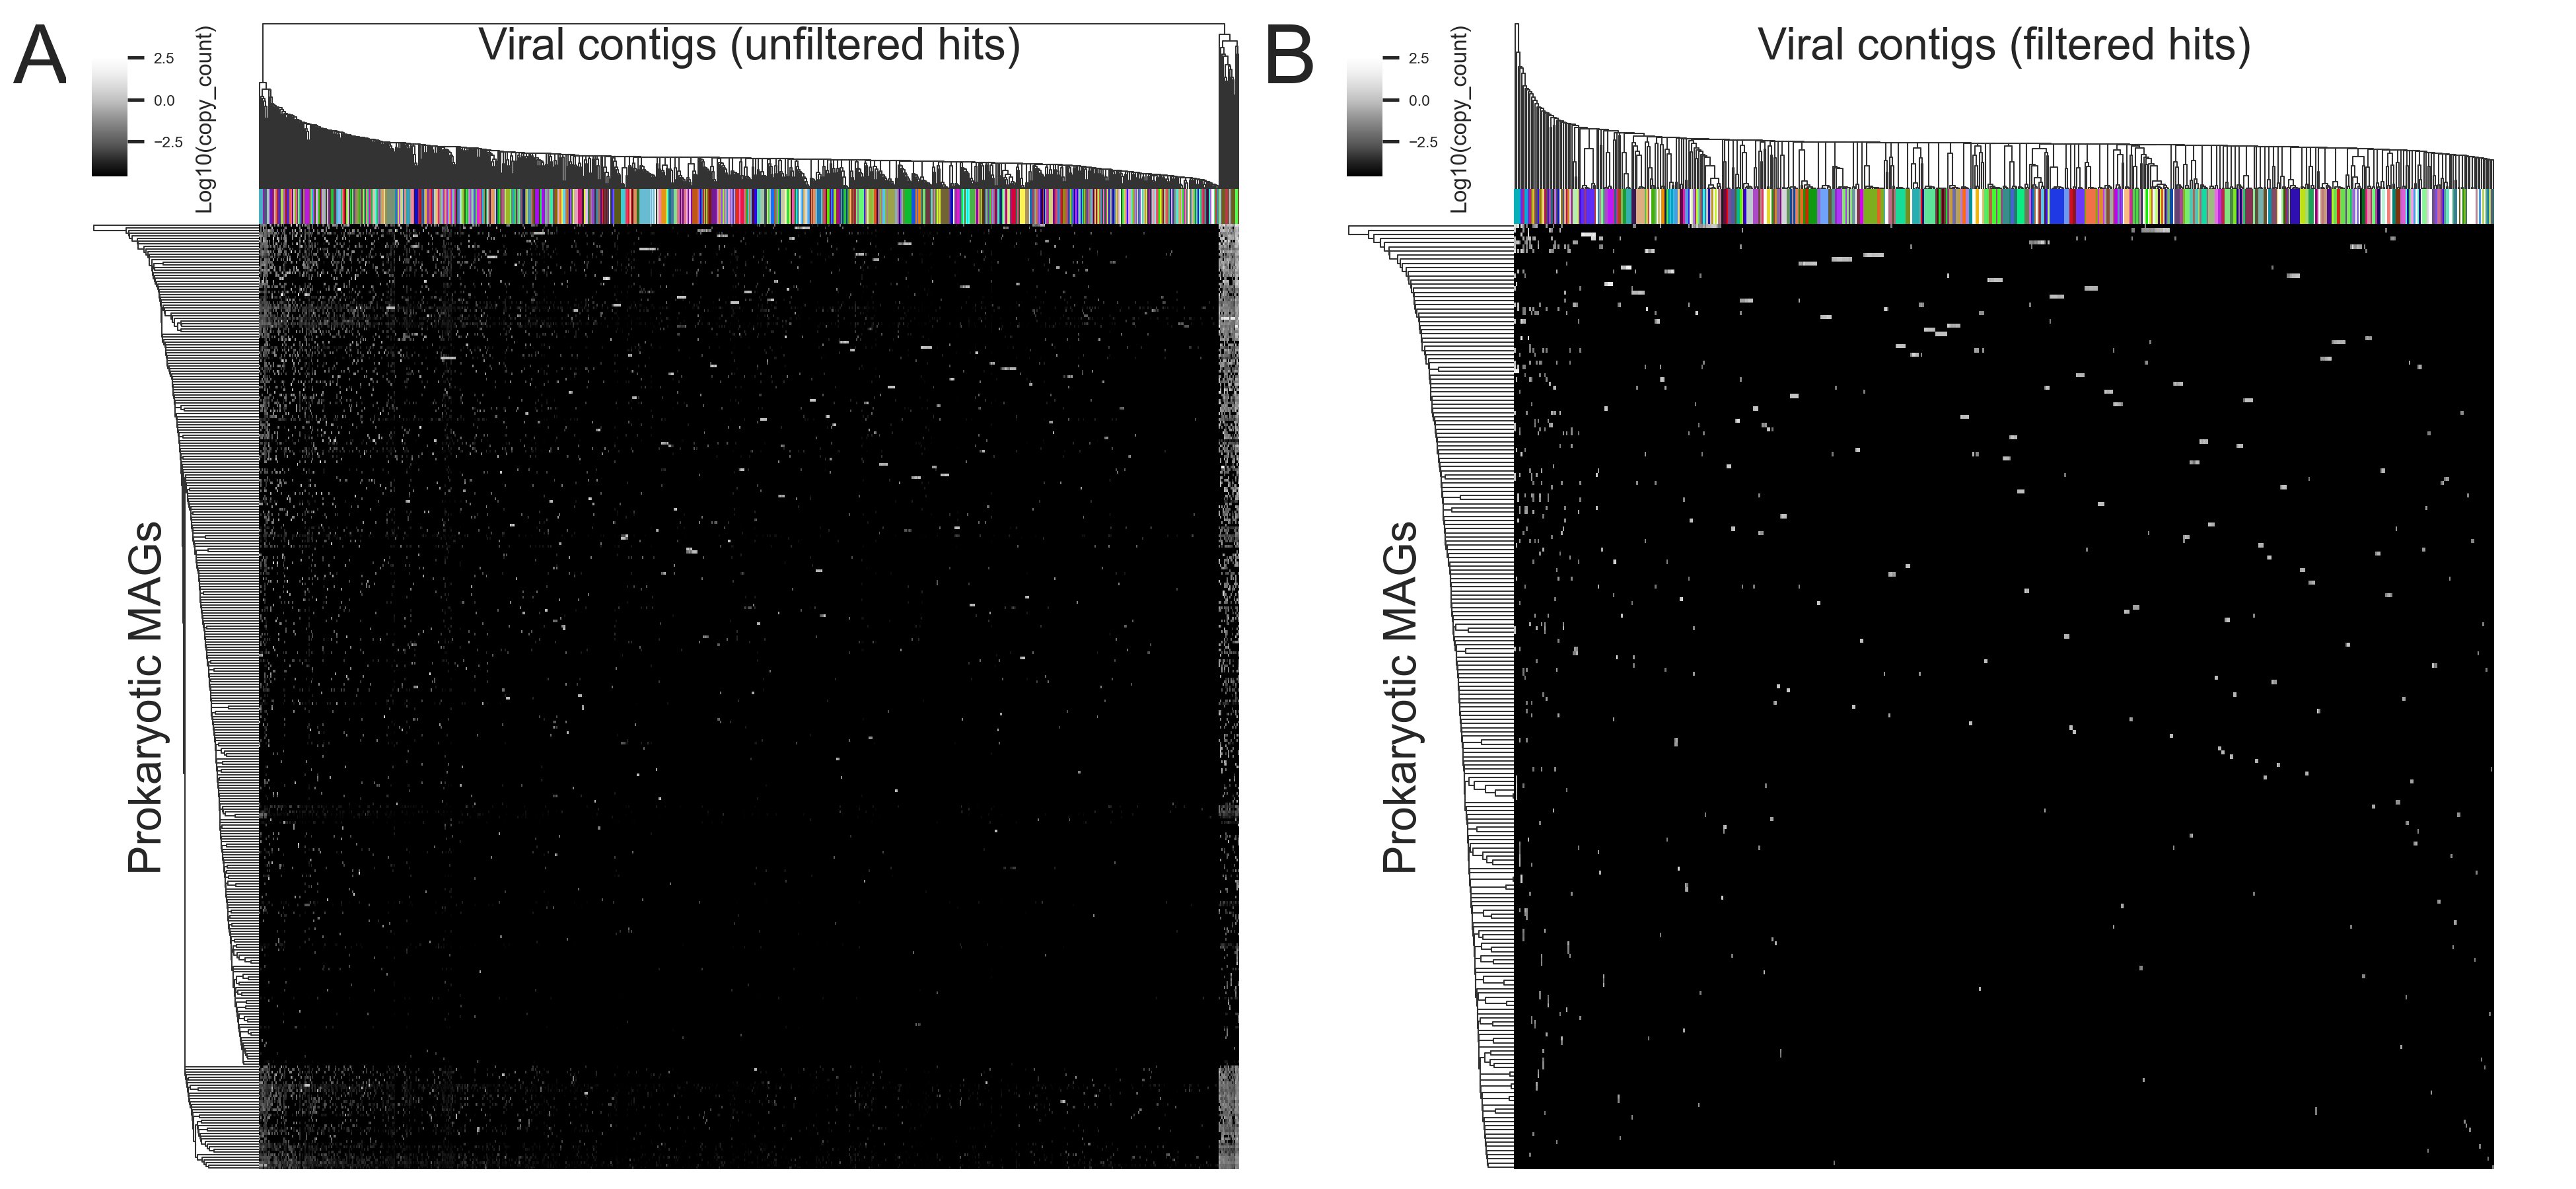
\includegraphics[width=\textwidth]{Figures/figure_contig_heatmaps.png}
\caption{\textbf{Viral contig host predictions.} Prokaryotic hosts identified for viral contigs from a sheep gut metagenome with ProxiPhage before (A) and after (B) thresholding. The color map represents the log of the estimated average copy count of each phage genome in its host. The colors above the phage contigs label the viral MAG that they belong to. Rows and columns are clustered according to linkage similarity with seaborn clustermap. Only viral contigs from viral MAGs are shown.}
\label{fig:figure_contig_heatmaps}
\end{figure*}
\newpage


\begin{figure*}[t]
\centering
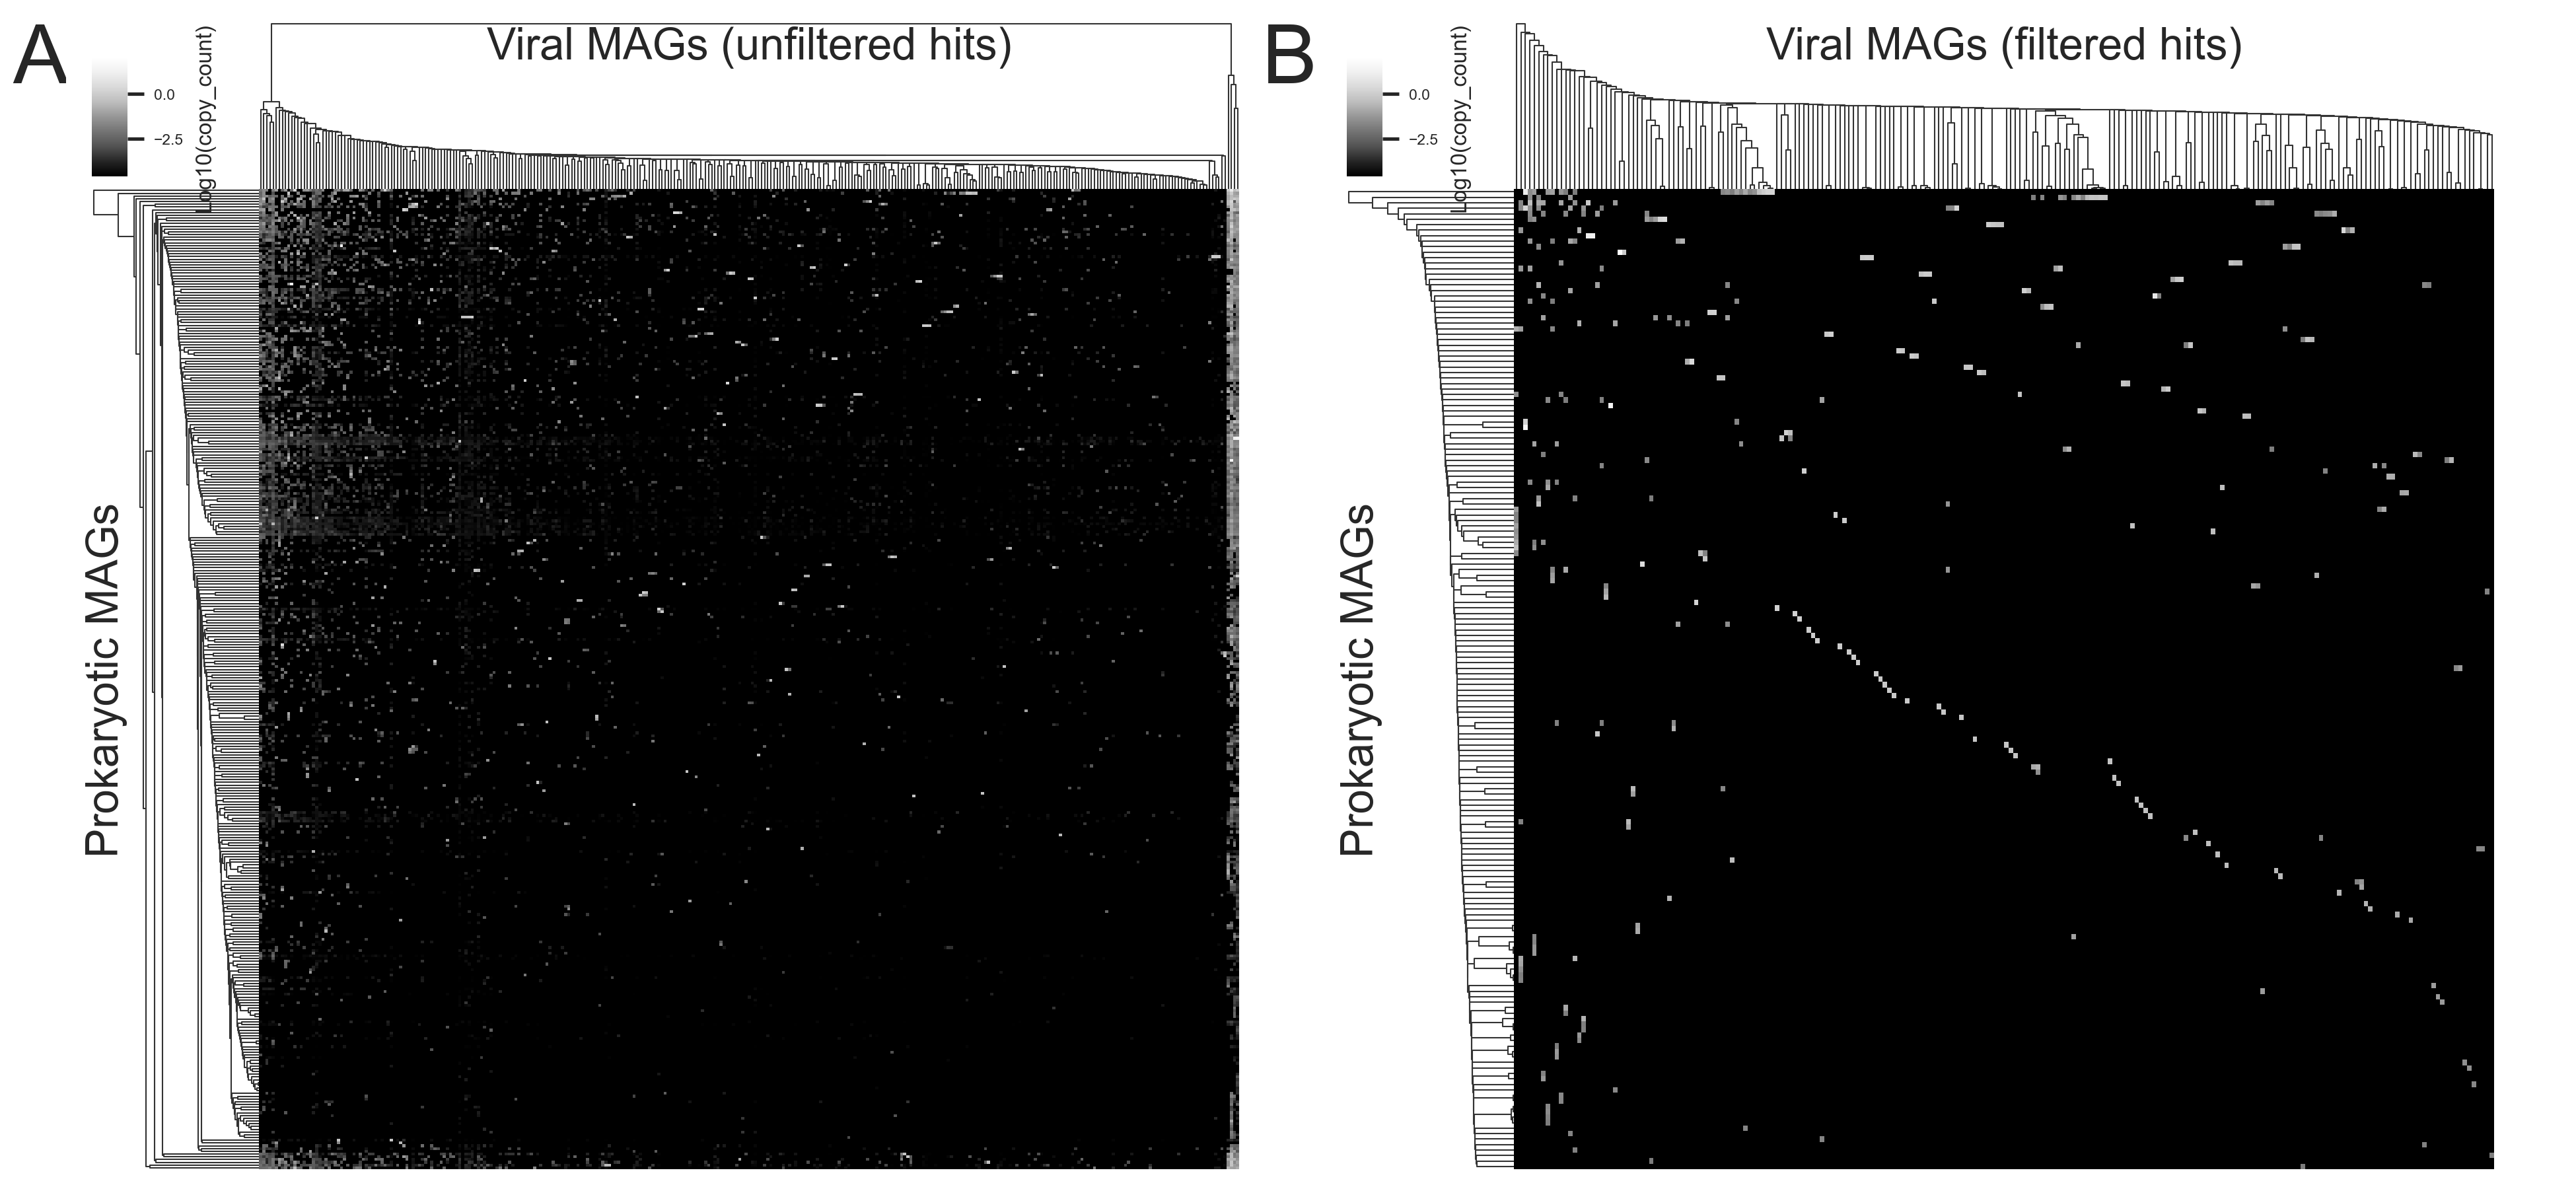
\includegraphics[width=\textwidth]{Figures/figure_cluster_heatmap.png}
\caption{\textbf{Viral MAG host predictions.} Prokaryotic hosts identified for viral MAGs from a sheep gut metagenome with ProxiPhage before (A) and after (B) thresholding. The color map represents the log of the estimated average copy count of each phage genome in its host. Rows and columns are clustered according to linkage similarity with seaborn clustermap.}
\label{fig:figure_cluster_heatmap}
\end{figure*}
\newpage
